\section{System Design}
\label{sec:design}

\begin{center}
\begin{figure*}[ht!]
 \centering
 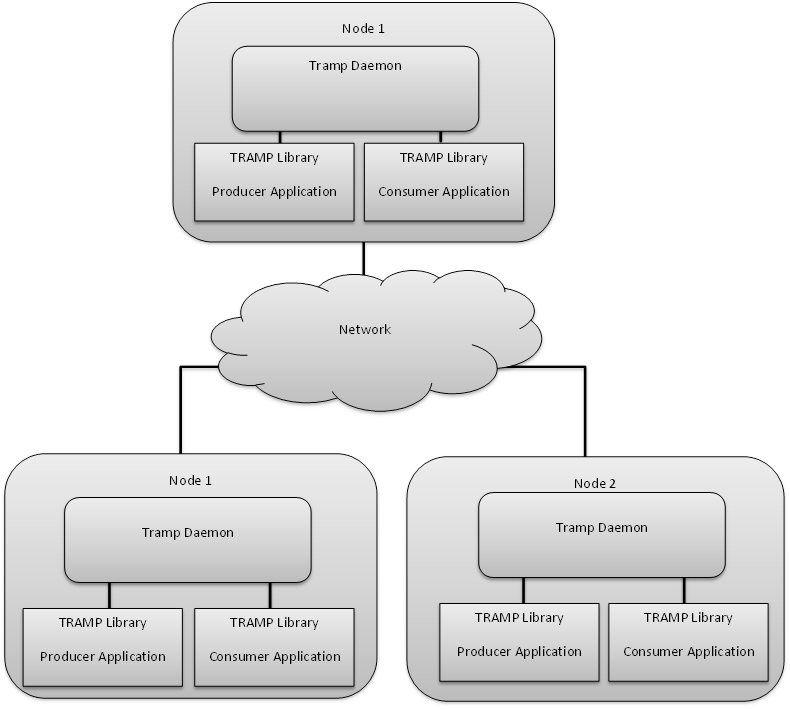
\includegraphics[width=6.0in, height=3.5in]{tramp_arch2.png}
 %img1.pdf: 0x0 pixel, 300dpi, 0.00x0.00 cm, bb=
\caption{The TRAMP Architecture}
\label{tramparc}
\end{figure*}
\end{center}

The TRAMP platform is a platform designed to stream real-time data from a device to other devices connected to the session, mobility is the keyword. Lets take the example given in the introduction; You are on a skype call with some of your friends when you find out you need to go out of the house. Traditionally you then had to end the skype call and call them up using your phone. The goal for TRAMP is to be able to seamlessly enter the conversation without your friend noticing you just changed device.

In TRAMP this is done by having a TRAMP daemon running on each device, with a consumer and a producer. The producer produces data, putting it into the shared memory, the TRAMP daemon then pushes the data to all other daemons connected to this session. When a TRAMP daemon gets data it puts it into the shared memory so the consumer can read it. All nodes has a TRAMP daemon, a producer and a consumer running. The shared memory of all nodes in the session are in synch (see Figure: \ref{tramparc}).

